\chapter{Fenomenolog\'ia}

%%%%%%%%%%%%%%%%%%%%%%%%%%%%%%%%%%%%%%%%%%%%%%%%%%%%%%%%%%%%%%%%%%%%%%%%%%%%%%%%
\section{Texturas}
Una teor\'ia m\'as fundamental que el modelo est\'andar deber\'ia permitir 
determinar $M_u$ y $M_d$ de una manera \'unica. Como las matrices de masa de los
quarks son de importancia fundamental es deseable obtener su estructura sin 
hacer suposiciones. El primer paso es determinar las matrices de masa a partir 
de datos experimentales. Evidentemente el paso anterior cuando mucho puede ser 
parcialmente exitoso, porque el conocimiento de los eigenvalores y los 
par\'ametros de mezcla no es suficiente para este prop\'osito. Un entendimiento 
profundo de la mezcla del sabor de los quarks y el fen\'omeno de la violaci\'on 
de $CP$, es deseable para estudiar las propiedades de las matrices de masa de 
los quarks $M_{u,d}$, cuyas texturas son totalmente desconocidas dentro del ME. 

Sin embargo, es posible hacer algunos progresos notando que las matrices de masa
pueden ser supuestas hermitianas, sin perder generalidad, para aquellas 
teor\'ias en las que no haya cambio de sabor en las corrientes de las parte 
derechas de los campos, como el modelo est\'andar. Como las partes 
derechas de los campos son singletes de $SU(2)$, siempre es posible escoger una 
base adecuada de los quarks parte derecha, que resulte en matrices de masa 
hermitianas. Una matriz de masa hermitiana general, $M_q$ (con $q=u $ o $ d$)
puede ser escrita como
$$
M_q=\left(\ba{ccc} E_q&A_q&F_q\\ A^*_q&D_q&B_q\\ F^*_q&B^*_q&C_q\ea\right),
$$
donde los elementos de la diagonal son reales y los elemento fuera de ella son
complejos.

En la mayor\'ia de los intentos por entender los modelos observados de las masas
y mezcla de los fermiones, se propone la existencia de una familia de simetr\'ia
abeliana o no abeliana, dejando una estructura especial del sabor en las 
matrices de Yukawa, que involucra texturas con ceros. En la b\'usqueda de las 
texturas de los ceros permitidos, se puede tomar la descripci\'on 
{\it bottom-up}, donde se usan los datos experimentales de las masas y mezcla de
los fermiones para derivar aquellas texturas de Yukawa que son permitidas por 
los experimentos.  

La textura con dos ceros de Fritzsch para la matriz hermitiana de masa de los 
quarks es 
\be
\label{matfrit}
{F2}=\matFritti,
\ee
como el elemento $V_{1,3}$ es el conjugado de $V_{3,1}$ ellos se cuentan como un
cero, y se puede obtener la textura con tres ceros de Fritzsch si se toma a 
$D=0$
\be\label{matfri}
{F3}=\matFrit,
\ee
donde $A$ y $B$ son elementos complejos y $C$ es un elemento real de la matriz 
de masas. Para obtener la textura de seis ceros de Fritzsch se toman matrices de
masa, tanto en el sector $u$ como en el $d$, de la forma de la matriz 
~(\ref{matfri}). Las texturas de cinco ceros se obtienen tomando el sector $u$ 
con la forma de ~(\ref{matfri}) o ~(\ref{matfrit}) y al sector $d$ con la forma 
de la matriz no escogida para el sector $u$, por lo tanto hay dos texturas de 
Fritzsch de cinco ceros.  

No existe ninguna justificaci\'on te\'orica para las matrices de masa  
propuestas por Fritzsch, por lo tanto, se vuelve esencial, desde el punto de 
vista fenomenol\'ogico, considerar matrices de masa de los quarks diferentes a 
las propuestas por Fritzsch ~\cite{Mah200901}. Las matrices diferentes a las de 
Fritzsch tienen los ceros en otros elementos de la matriz de masa. 
{\tiny
\begin{table}[h!]\label{t2}
\begin{scriptsize}
\caption{Matrices de { masa} hermitianas de los quarks con consistencia 
fenomenol\'ogica seg\'un Ramond, Robert y Ross ~\cite{rrr}.}
$$\ba{c|ccccc}\hline\hline
\mbox{ RRR} & I & II & III & IV & V\\ \hline \\
M_u&\left(\ba{ccc} 0&A&0\\ A*&D&0\\ 0&0&C \ea\right) & 
\left(\ba{ccc} 0&A&0\\ A*&0&B\\ 0&B*&C \ea\right) & 
\left(\ba{ccc} 0&0&F\\ 0&D&0\\ F*&0&C \ea\right) & 
\left(\ba{ccc} 0&A&0\\ A*&D&B\\ 0&B*&C \ea\right) & 
\left(\ba{ccc} 0&0&F\\ 0&D&B\\ F*&B*&C \ea\right)\\  \\ \hline\\
M_d&\left(\ba{ccc} 0&A&0\\ A&D&B\\ 0&B&C \ea\right) & 
\left(\ba{ccc} 0&A&0\\ A*&D&B\\ 0&B*&C \ea\right) & 
\left(\ba{ccc} 0&A&0\\ A*&D&B\\ 0&B*&C \ea\right) & 
\left(\ba{ccc} 0&A&0\\ A*&D&0\\ 0&0&C \ea\right) & 
\left(\ba{ccc} 0&A&0\\ A*&D&0\\ 0&0&C \ea\right)\\  \\ \hline
\ea $$
\end{scriptsize}
\end{table}
}
Ramond, Robert y Ross (RRR) ~\cite{rrr} propusieron matrices sim\'etricas o 
hermitianas para buscar estructuras en los acoplos de Yukawa de los quarks que 
estuvieran en acuerdo con los datos experimentales. En su investigaci\'on ellos
trabajaron con texturas de cinco y seis ceros y encontraron cinco texturas de
cinco ceros que eran consistentes con los experimentos, \'estas se muestran en
la tabla 3.1.
%~\ref{t2}.

\subsection{Maximal en el invariante de Jarlskog}
Aunque hay muchas versiones diferentes de la hip\'otesis del maximal en la 
violaci\'on de $CP$, la versi\'on convencional demanda que la naturaleza tome un
valor en la fase de la violaci\'on de $CP$ tal que el invariante de Jarlskog,
$J$, tome su valor m\'aximo ~\cite{Koi200401}.

Como en el modelo est\'andar solo hay una fuente de la violaci\'on de $CP$, que
es la fase $\delta$ de violaci\'on de $CP$, en consecuencia, todos los 
observables de la violaci\'on de $CP$ est\'an fuertemente correlacionados. Desde
el punto de vista de la teor\'ia fundamental de los quarks esta situaci\'on no
es satisfactoria y es de inter\'es ver el origen te\'orico de la fase $\delta$ 
de la matriz de mezcla. En el a\~no 2001 se hizo un trabajo ~\cite{Rod200101} 
con el prop\'osito de mostrar que el maximal en el invariante de Jarlskog, $J$, 
y el maximal en la fase de la violaci\'on de $CP$ son fenomenol\'ogicamente 
permitidos. El invariante de Jarlskog, $J$, est\'a relacionado a la violaci\'on 
de $CP$ y es funci\'on de la fases de violaci\'on, $\delta$. Es bien conocido 
que el invariante de Jarlskog $J$ se obtiene de las matrices de masa de los 
quarks $M_q$. A partir de imponer la condici\'on de maximal al invariante de 
Jarlskog y a la fase de la violaci\'on de $CP$ se obtiene que las matrices de 
Ramond que cumplen con dichas condiciones son los modelos I, III, IV y V 
~\cite{Rod200101}.


Normalmente se dice que cualquiera de las convenci\'ones de fase de la matriz de
Cabibbo-Kobayashis-Maskawa ($V_{ckm}$) son equivalentes entre s\'i, por la 
invariancia ante refasamiento. Esto es verdad para todas las cantidades 
observables. Sin embargo, las matrices de masa de los quarks ($M_u,M_d$) no son
invariantes de refasamiento, aunque \'estas son invariantes ante cambios de 
base: $M_u\rightarrow M'_u=A^{\dag}M_uB_u$, 
$M_d\rightarrow M'_d=A^{\dag}M_dB_d$. A veces la invariancia de refasamiento se
confunde con la invariancia de cambio de bases. El par\'ametro $\delta$ de la
violaci\'on de $CP$ en la mariz $V_{ckm}$ no es observable, y depende de la
convenci\'on de fase. Las cantidades observables relacionadas a la violaci\'on
de $CP$ son los \'angulos ($\phi_1, \phi_2,\phi_3$)=($\beta,\alpha,\gamma$) en los tri\'angulos unitarios. Cuando se
toma una convenci\'on de fases, el par\'ametro $\delta$ se vuelve observable.
Las predicciones  basadas en la hip\'otesis de m\'axima violaci\'on de $CP$ 
pueden ser obtenidas exitosamente solo cuando se adoptan las convenciones de 
fase original, de Kobayashi-Maskawa, y la de Fritzsch-Xing ~\cite{Koi200601}.

%%%%%%%%%%%%%%%%%%%%%%%
Por ejemplo, considerando una matriz de mezcla, $V_{ckm}$, dada como
\be\label{2.1}
V=V(i,j)\equiv R^T_iP_jR_jR_k\qquad (i\neq j\neq k),
\ee
donde las $R_i$ son definidas por
$$
R_1(\theta)=\left(\ba{ccc} 1&0&0\\0&c&s\\0&-s&c\ea\right), \qquad
R_2(\theta)=\left(\ba{ccc} c&0&s\\0&1&0\\-s&0&c\ea\right), \qquad
R_3(\theta)=\left(\ba{ccc} c&s&0\\-s&c&0\\0&0&1\ea\right), 
$$
con $s=\sen\theta$ y $c=\cos\theta$, y las $P_i$ est\'an dadas por 
$P_1=\mbox{diag}(e^{i\delta},1,1) $, $P_2=\mbox{diag}(1,e^{i\delta},1)$ y 
$P_3=\mbox{diag}(1,1,e^{i\delta})$, es posible obtener la convenci\'on de fase 
original, la convenci\'on de Kobayashi-Maskawa, a partir de $V(1,1)$
$$
V_{km}=R^T_1(\theta_2)P_3(\delta_{km}+\pi)R_3(\theta_1)R_1(\theta_3)
$$
\be\label{cfkm}
=\left(\ba{ccc}c_1&-s_1c_3&-s_1s_3\\ s_1c_2&c_1c_2c_3-s_2s_3e^{i\delta_{km}}&
c_1c_2s_3+s_2c_3e^{i\delta_{km}}\\
 s_1s_2&c_1s_2c_3+c_2s_3e^{i\delta_{km}}&c_1s_2s_3-c_2c_3e^{i\delta_{km}}
\ea\right),
\ee
entonces, la cantidad invariante $J$ est\'a dada por 
\be\label{invJcfkm}
J=c_1s^2_1c_2s_2c_3s_3\sen\delta_{km},
\ee
es decir
\be\label{1.19}
J=\frac{|V_{11}||V_{12}||V_{13}||V_{21}||V_{31}|}{1-|V_{11}|^2}\sen\delta_{km},
\ee
y se necesita, para obtener un maximal, que $\delta_{km}=\frac{\pi}{2}$.

%La convenci\'on de fase propuesta por Fritzsch y Xing en 1997 puede ser obtenida
%de la expresi\'on $V(3,3)$, y de forma expl\'icita est\'a dada por
%$$
%V(3,3)=R^T_3(\theta^u_{12})P_1(\delta)R_1(\theta_{23})R_3(\theta^d_{12})
%$$
%\be\label{v33}
%V(3,3)=\left(\ba{ccc} e^{i\delta}c^u_{12}c^d_{12}+c_{23}s^u_{12}s^d_{12}&
%e^{i\delta}c^u_{12}s^d_{12}-c_{23}s^u_{12}c^d_{12}&-s_{23}s^u_{12}\\
%e^{i\delta}s^u_{12}c^d_{12}-c_{23}c^u_{12}s^d_{12}&
%e^{i\delta}s^u_{12}s^d_{12}+c_{23}c^u_{12}c^d_{12}& s_{23}c^u_{12}\\
%-s_{23}s^d_{12}&-s_{23}c^d_{12}&c_{23}\ea\right).
%\ee
%Para la expresi\'on ~(\ref{v33}), se tiene la forma del invariante $J$ como
%\be\label{invJcffx}
%J=c_{23}s^2_{23}c^u_{12}s^u_{12}c^d_{12}s^d_{12}\sen\delta=
%\frac{|V_{13}||V_{23}||V_{33}||V_{32}||V_{31}|}{1-|V_{33}|^2}\sen\delta.
%\ee


%%%%%%%%%%%%%%%%%%%%%%%%%%%%%%%%%%%%%%%%%%%%%%%%%%%%%%%%%%%%%%%%%%%%%%%%%5
\section{Datos experimentales}
La \'unica manera para que el ME sea consistente con los datos experimentales, 
relacionados a la violaci\'on de la simetr\'ia discreta $CP$, es que la matriz
$V_{ckm}$ sea compleja, ya que el \'unico t\'ermino de la lagrangiana del ME
que puede no respetar la simetr\'ia $CP$ es el de las corrientes cargadas. 
La fenomenolog\'ia de las interacciones electrod\'ebiles asegura que la matriz 
$V_{ckm}$ es compleja y unitaria. $V_{ckm}$ puede ser parametrizada por nueve 
par\'ametros (o en general por $n^2_g$ par\'ametros, donde $n_g$ es el n\'umero 
de familias). Pero se sabe de la mec\'anica cu\'antica que la fase de una 
funci\'on de onda no es una cantidad medible; por este motivo, se debe examinar
cu\'ales fases son medibles y cu\'ales no tienen sentido f\'isico en la matriz 
de mezcla, $V_{ckm}$. Es posible absorber o cambiar cinco par\'ametros
($2n_g-1$) a partir de las fases de los quarks, adem\'as pueden ser 
parametrizados tres \'angulos de rotaci\'on ($\frac{1}{2}n_g(n_g-1)$), los 
\'angulos de Euler. As\'i, el resto de los par\'ametros de la matriz $V_{ckm}$,
a los que se les llaman fases, es uno ($n_{fase}=\frac{1}{2}(n_g-2)(n_g-1)$) y 
es esta fase la que proporciona la violaci\'on de $CP$ en el modelo est\'andar.
Esto no significa que la violaci\'on de $CP$ es entendida; solamente se ha 
encontrado una forma econ\'omica y fenomenol\'ogicamente exitosa de agregar la
violaci\'on de $CP$ en el modelo est\'andar ~\cite{Big200101}. Para dos familias
no es posible obtener violaci\'on de $CP$ con la descripci\'on que se acaba de
hacer, pero existen otros modelos con implicaciones de las cuales la violaci\'on
de $CP$ puede ser obtenida, por ejemplo, extendiendo el sector del Higgs la
violaci\'on de $CP$ es asociada al rompimiento espont\'aneo de simetr\'ia 
~\cite{Jar198901}.

Las cantidades con significado f\'isico deben ser invariantes bajo un cambio de
fase de los campos de los quarks; solo funciones de $V_{ckm}$ que sean 
invariantes ante refasamiento pueden ser medibles. Los invariantes m\'as simples
son los m\'odulos de los elementos de matriz, denotados por
$$U_{\alpha i}\equiv\left|V_{\alpha i}\right|^2.$$

Experimentalmente, las funciones invariantes ante cambio de fase de la matriz
$V_{ckm}$ para las cuales se tiene acceso m\'as directo, tambi\'en son los 
m\'odulos de sus elementos de matriz. Los valores experimentales actuales 
\cite{Nak201001} se presentan en la tabla 3.2.%~\ref{pdgvckm}.
{\tiny
\begin{table}[h!]\label{pdg}
\begin{scriptsize}
\caption{Valores experimentales de los m\'odulos de la matriz de mezcla.} 
$$\ba{c|c} \hline \hline
|V_{ckm}|&\mbox{Exp}\\ \hline
|V_{ud}|&0.97425\pm0.00022\\
|V_{us}|&0.2252\pm0.0009  \\
|V_{cd}|&0.230\pm0.011    \\
|V_{cs}|&1.023\pm0.036    \\
|V_{ub}|&(3.89\pm0.44)\times10^{-3} \\
|V_{cb}|&(40.6\pm1.3)\times10^{-3}  \\
|V_{td}|&(8.4\pm0.6)\times10^{-3}   \\
|V_{ts}|&(38.7\pm2.1)\times10^{-3}  \\
|V_{tb}|&0.88\pm0.07     \\ \hline
\ea
$$
\end{scriptsize}
\end{table}
}
%$$|V_{ud}|=0.97425\pm0.00022.$$ 
%Tres m\'etodos diferentes se han usado en su determinaci\'on, siendo el 
%estudio del decaimiento nuclear beta el m\'as preciso. La magnitud de $|V_{us}|$
%es tradicionalmente obtenido del decaimiento semilept\'onico del kaon; 
%tambi\'en es posible hacerlo a partir de los decaimientos lept\'onicos del kaon,
%del hiper\'on y del $\tau$. El valor promedio determinado es
%$$|V_{us}|=0.2252\pm0.0009$$
%La forma m\'as precisa para determina $|V_{cd}|$ esta basada en la 
%interacci\'on neutrino-antineutrino. El valor reportado es
%$$|V_{cd}|=0.230\pm0.011.$$
%Es posible determinar $|V_{cs}|$ de los decaimientos semilept\'onicos $D$ y 
%lept\'onicos $D_s$, siendo
%$$|V_{cs}|=1.023\pm0.036$$
%el valor. Los valor reportados para $|V_{cb}|$ y $|V_{ub}|$ se extraen de los 
%decaimiento $B$ y son
%$$|V_{ub}|=(3.89\pm0.44)\times10^{-3},$$
%$$|V_{cb}|=(40.6\pm1.3)\times10^{-3}.$$
%Los m\'odulos de la matriz de mezcla $|V_{td}|$ y $|V_{ts}|$ 
%no pude ser medidos del decaimiento a nivel de \'arbol del quark t, as\'i que se
%tienen que usar las oscilaciones $B^0_{d,s}-\bar B^0_{d,s}$, obteniendo
%$$|V_{td}|=(8.4\pm0.6)\times10^{-3}$$
%$$|V_{ts}|=(38.7\pm2.1)\times10^{-3}.$$
%La determinaci\'on directa de $|V_{tb}|$ se volvi\'o posible de la secci\'on 
%transversal en la producci\'on de quarks t, teniendo un valor
%de 
%$$|V_{tb}|=0.88\pm0.07.$$
Se observa que el valor central de $|V_{cs}|$ es mayor a 1, por lo tanto,
podr\'ia viola la unitariedad de la matriz de mezcla. Los elementos de la matriz
de mezcla pueden determinarse de mejor manera si adem\'as se utilizan las
restricciones impuestas por el ME. Las restricciones impuestas por la
unitariedad para tres generaciones reduce el intervalo permitido para los
elementos de la matriz de mezcla y son los siguientes ~\cite{Nak201001}
\be\label{pdgvckm}
|V_{ckm}|=\left(\ba{ccc} 0.97428\pm0.00015&0.2253\pm0.0007&
0.00347^{+0.00016}_{-0.00012}\\
0.2252\pm0.0007&0.97345^{+0.00015}_{-0.00016}&0.0410^{+0.0011}_{-0.0007}\\
0.00862^{+0.00026}_{-0.00020}&0.0403^{+0.0011}_{-0.0007}&0.999152^{+0.000030}
_{-0.000045}\ea\right).
\ee


Los siguientes invariantes, en orden de simplicidad, son los cuartetos,
$$
Q_{\alpha i\beta j}\equiv V_{\alpha i}V_{\beta j}V^*_{\alpha j}V^*_{\beta i},
$$
donde se pide que $\alpha\neq\beta$ y $i\neq j$, para que el cuarteto no se 
reduzca al producto de dos m\'odulos al cuadrado. En general, la violaci\'on de 
$CP$ existe si cualquiera de las funciones de $V_{ckm}$ invariantes ante
refasamiento no es real ~\cite{Bra199901}.

Como la matriz de mezcla de los quarks, $V_{ckm}$, es unitaria 
$$V_{ckm}V^{\dag}_{ckm}=V^{\dag}_{ckm}V_{ckm}=1$$
se pueden obtener seis relaciones de ortogonalidad, tres relaciones de pares de
renglones diferentes y tres de pares de diferentes columnas,
$$
V^{\dag}_{ckm}V_{ckm}= 
\left(\ba{ccc} V^*_{ud}&V^*_{cd}&V^*_{td}\\
V^*_{us}&V^*_{cs}&V^*_{ts}\\ V^*_{ub}&V^*_{cb}&V^*_{tb}\ea\right)
\left(\ba{ccc} V_{ud}&V_{us}&V_{ub}\\
V_{cd}&V_{cs}&V_{cb}\\ V_{td}&V_{ts}&V_{tb}\ea\right)
=\left(\ba{ccc} 1&0&0\\0&1&0\\0&0&1\ea\right),
$$
por ejemplo, del primer rengl\'on y la segunda columna se obtiene
\be\label{tu}
V_{ud}V^*_{cd}+V_{us}V^*_{cs}+V_{ub}V^*_{cb}=0.
\ee
Multiplicando a la ecuaci\'on ~(\ref{tu}) por $V^*_{us}V_{cs}$,
$$
V^*_{us}V_{cs}V_{ud}V^*_{cd}+V^*_{us}V_{cs}V_{us}V^*_{cs}+V^*_{us}V_{cs}V_{ub}
V^*_{cb}=0
$$
y tomando la parte imaginaria, se obtiene
$$ \mbox{Im}Q_{udcs}=-\mbox{Im}Q_{ubcs},$$
se concluye que los cuartetos $Q_{udcs}$ y $Q_{ubcs}$ tienen partes imaginarias
sim\'etricas. De manera equivalente, con el resto de los pares de renglones
diferentes y los pares de columnas diferentes, se concluye que la parte 
imaginaria de los cuartetos a lo m\'as difiere por un signo. De esta manera se
define el invariante de Jarlskog
\be\label{idj}
J\equiv \mbox{Im}Q_{uscb}=\mbox{Im}(V_{us}V_{cb}V^*_{ub}V^*_{cs}),
\ee
sabiendo que la parte imaginaria  de todos los cuartetos es igual a $J$, o con
signo distinto. El valor experimental para el invariante de Jarlskog es 
~\cite{Nak201001}
$$J=(2.91^{+0.19}_{-0.11})\times10^{-5}.$$

La relaci\'on de ortogonalidad ~(\ref{tu}) puede ser interpretada como un
tri\'angulo en el plano complejo. Sin embargo el tri\'angulo unitario que se usa
com\'unmente surge de la ecuaci\'on
\be\label{nanana}
V_{ud}V^*_{ub}+V_{cd}V^*_{cb}+V_{td}V^*_{tb}=0,
\ee
ver figura 3.1. Los 6 tri\'angulos,
uno por cada relaci\'on de ortogonalidad, son rotados cuando la matriz de mezcla
de los quarks, $V_{ckm}$, sufre un cambio de fase. Sin embargo, la forma de los
tri\'angulos permanece sin cambios, ya que los \'angulos internos y las
longitudes de los lados son invariantes ante el refasamiento.
%%%%%%%%%%%%%%%%%%%%%%%%%%%%%%%%%%%%%%%%%%%%%%%%%%5555
\begin{figure}\label{fig2}
\centering
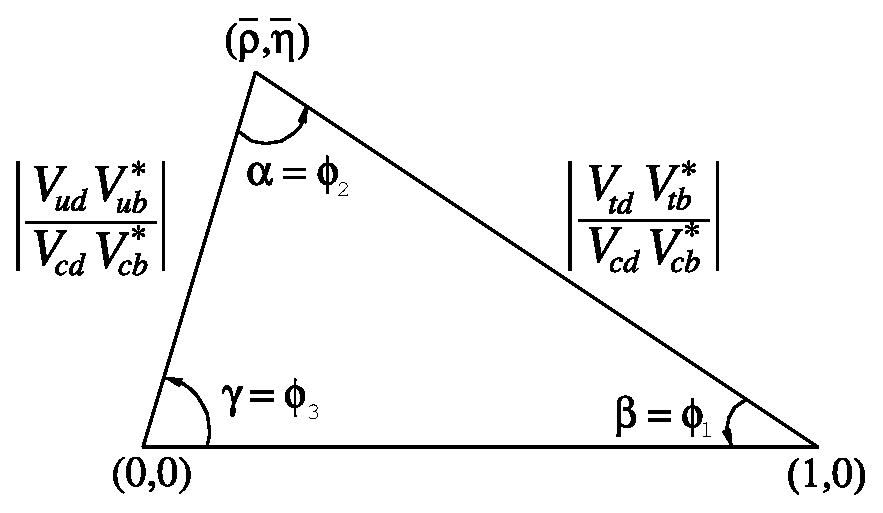
\includegraphics[height=8cm,angle=0]{triangle2.eps}
\caption{Tri\'angilo unitario en el plano complejo ~\cite{Nak201001}.}
\end{figure}
%%%%%%%%%%%%%%%%%%%%%%%%%%%%%%%%%%%%%%%%%%%%%%%%%%%%%%
Si se divide ~(\ref{nanana}) entre $V_{cd}V^*_{cb}$ se obtiene
$$
\frac{V_{ud}V^*_{ub}}{V_{cd}V^*_{cb}}+1+\frac{V_{td}V^*_{tb}}{V_{cd}V^*_{cb}}=0,
$$
en donde los \'angulos internos del tri\'angulo que se forma est\'an definidos 
como el argumento de n\'umeros complejos, dados de la siguiente manera
\be\label{alpha}
\alpha\equiv \mbox{arg}\left(-\frac{V_{td}V^*_{tb}}{V_{ud}V^*_{ub}}\right)
\ee
\be\label{beta}
\beta\equiv \mbox{arg}\left(-\frac{V_{cd}V^*_{cb}}{V_{td}V^*_{tb}}\right)
\ee
\be\label{gamma}
\gamma\equiv \mbox{arg}\left(-\frac{V_{ud}V^*_{ub}}{V_{cd}V^*_{cb}}\right),
\ee
y los valores experimentales son ~\cite{Nak201001}
$$\alpha=(88^{+6}_{-5}),$$
$$\sin{2\beta}=0.681\pm{0.025},$$
y
$$\gamma=77^{+30}_{-32}.$$

Una vez definidos los tri\'angulos, al invariante de Jarlskog se le 
puede dar la interpretaci\'on geom\'etrica del doble del \'area de los 
tri\'angulos
$$
A=\frac{|\mbox{Im} Q_{udcb}|}{2}=\frac{|J|}{2}. 
$$
As\'i, aunque los tri\'angulos tienen diferentes formas, el \'area de ellos es
la misma, $\frac{|J|}{2}$. Como los cuartetos son las funciones m\'as simples de
$V_{ckm}$ que pueden ser no reales, si $J$ es diferente de cero la violaci\'on 
de $CP$ existe, si es cero no hay violaci\'on y los tri\'angulos se colapsan a
una l\'inea y su \'area es cero.
%%%%%%%%%%%%%%%%%%%%%%%%%%%%%%%%%%%%%%%%%%%%%%%%%%%%%%%%%%%%%%%%%%%%%%%%%%%%%%%%
%%%%%%%%%%%%%%%%%%%%%%%%%%%%%%%%%%%%%%%%%%%%%
\subsection{Transformaciones de base d\'ebil, el trabajo de Branco y 
Emmanuel-Costa}

Branco y Emmanuel-Costa demostraron que siempre es posible hacer una 
transformaci\'on de base d\'ebil tal que las matrices de masa de los quarks sean
hermitianas y ambas presenten texturas de ceros en el elemento $(1,1)$, teniendo
la forma
\be\label{emI}
M_u=\left(\ba {lcr} 0&*&*\\ *&*&*\\ *&*&* \ea \right),\qquad 
M_d=\left(\ba {lcr} 0&*&*\\ *&*&*\\ *&*&* \ea \right).
\ee 
A partir de ~(\ref{emI}) intentaron llegar a texturas de cuatro ceros. Su 
motivaci\'on radicaba en el problema mostrado por las texturas de m\'as ceros 
en la reproducci\'on de datos fenomenol\'ogicos. La conclusi\'on a la que 
llegaron fue que en general no es posible obtener texturas de cuatro ceros a
partir de transformaciones de base d\'ebil, solo unas cuantas son accesibles.
Entre las texturas accesibles estaba aquella en la que ambas matrices de masa
ten\'ian ceros en $(1,1)$ y $(1,3)$, de la forma de las matrices con dos ceros
de Fritzsch ~(\ref{matfrit}) ~\cite{Bra199902}.

En trabajos posteriores Branco y colaboradores investigaron la dificultad que
presentaban algunas texturas al intentar determinar de manera precisa los 
\'angulos $\beta\equiv \mbox{arg}(-\frac{V_{cd}V^*_{cb}}{V^*_{td}V_{tb}})$ y
$\gamma\equiv \mbox{arg}(-\frac{V_{ud}V^*_{ub}}{V^*_{cd}V_{cb}})$ invariantes 
ante refasamiento ~\cite{Bra200401}. Una manera de resolver dicha discrepancia 
con los datos del \'angulo $\beta$ es proponer fases no factorizables, en al 
menos una matriz de masa. Para ellos la raz\'on era f\'acil de entender, la 
contribuci\'on de tal fase permit\'ia alcanzar los valores del $\sen2\beta$ 
demasiados grandes para la gran mayor\'ia de las texturas. Adem\'as, encontraron
la condici\'on necesaria para la existencia de fases no factorizables: las 
texturas no deben presentar ceros en elementos que no sean de la diagonal. Con 
esta condici\'on, ninguna textura de Fritzsch o las cinco propuestas por Ramond pueden presentar fases no factorizables. 

Siguiendo con la misma t\'onica, investigaron c\'omo los trabajos que 
propon\'ian nueva f\'isica afectaban a los datos que se utilizan como criterio
en la aceptaci\'on de alguna textura, en particular, otra vez, los \'angulos 
$\beta$ y $\gamma$. Su trabajo se bas\'o en texturas en las que no pudieran 
haber fases no factorizables. Clasificaron a las texturas dependiendo del 
\'angulo en el que presentaban problemas a la hora de reproducirlo. En el 
estudio del impacto de nueva f\'isica (NF) en las pruebas de las texturas de 
Yukawa, se tienen que especificar cu\'ales son la suposiciones de la naturaleza
de la NF. En la mayor\'ia de los escenarios de NF considerados en la literatura,
usualmente se asume que la NF no contribuye significativamente a  nivel de 
\'arbol en los decaimientos de {\it strange} y mesones $B$. Esto implica que la
NF no afecta los resultados de $|V_{su}|$, $|V_{cb}|$, $|V_{ub}|$ y $\gamma$ en
los datos experimentales. Utilizando estos cuatro datos, se puede reconstruir la
matriz de mezcla $V_{ckm}$ y los tri\'angulos unitarios. Sin embargo, se puede 
proponer que hay contribuciones apreciables por parte de la NF a las mezclas de
$B^0_d-\bar B^0_d$ y $B^0_s-\bar B^0_s$, as\'i los datos experimentales de 
$V_{td}$, $V_{ts}$ y $\beta$ son afectados. A la conclusi\'on que se llega en 
dicha investigaci\'on es que si una textura particular predice un valor de 
$\beta$ o de $|V_{td}|$ en desacuerdo con los datos experimentales, se puede 
justificar por la presencia de nueva f\'isica en la mezcla $B^0_d-\bar B^0_d$. 
Sin embargo, no se pueden justificar texturas que no den resultados correctos 
para $\frac{|V_{ub}|}{|V_{cb}|}$ o para $\gamma$. Esto es importante porque la 
mayor\'ia de las texturas de Yukawa tienen dificultad en obtener estos datos 
~\cite{Bra200601}.

En un trabajo m\'as reciente ~\cite{Emm200901} se concluy\'o que no es posible 
obtener texturas de cuatro ceros a partir de transformaciones de base d\'ebil.
Partiendo de ~(\ref{emI}) es posible agregar un cero extra al sector $d$ sin
modificar los ceros exactos de las texturas. Observando que a\'un hay un 
excedente de par\'ametros, se intenta obtener otro cero a partir de 
transformaciones de base d\'ebil, como ya se hab\'ia hecho a\~nos atras 
~\cite{Bra199902}, pero tomando en cuenta los datos experimentales recientes. 
Con \'estos, hicieron una variaci\'on aleatoria de todos los posibles valores 
permitidos de las masas de los quarks y los cuatro par\'ametros de la matriz de
mezcla $V_{ckm}$. Entonces, encontraron que tal transformaci\'on no es posible,
as\'i que la suposici\'on de cualquier cero adicional tiene implicaciones 
f\'isicas. Se pueden derivar todos los pares de $M_u$ y $M_d$ (quince pares en
total) que tienen un cero en la misma posici\'on en la diagonal para ambos 
sectores  y un cero adicional en el sector $d$. Tambi\'en se pudiera tener un
cero extra en el sector $u$ en lugar de el sector $d$, teniendo un total de
treinta pares de texturas de ceros de base d\'ebil ~\cite{Emm200901}. Ya que no
existe ninguna justificaci\'on para  
imponer que las matrices de masa sean hermitianas, tambi\'en obtuvieron que 
el n\'umero m\'aximo de ceros en las matrices de masa no hermitianas, que pueden
ser obtenidas a partir de transformaciones de bases d\'ebil, son nueve. Fritzsch
ya hab\'ia propuesto texturas de ceros a matrices de masa no hermitianas 
clasific\'andolas en tres tipos: interacci\'on de vecinos cercanos, matrices 
tri\'angular y matrices de fase ~\cite{Fri200001}. 


%%%%%%%%%%%%%%%%%%%%%%%%%%%%%%%%%%%%%%%%%%%%%%%%%%%%%%%%%%%%%%%%%%%%%%%%%5
\section{Metodolog\'ia}
Las masas de los quarks son los eigenvalores de la matriz de masa de los quarks,
las cuales son introducidas en el modelo est\'andar por el acoplo de los campos
de los quarks con el campo escalar. En el presente trabajo se utilizan tres 
diferentes c\'alculos de los intervalos de las masas a escala electrod\'ebil y 
son presentadas en la tabla 3.3.
%~\ref{t3masas}. 
Estos valores se utilizan para 
calcular la matriz $V_{ckm}$ te\'orica que se obtiene al diagonalizar texturas
en las matrices de masa de los quarks y deben compararse los datos 
experimentales de la mezcla de los quarks y la violaci\'on de $CP$.
\begin{table}[h!]\label{t3masas}
\begin{footnotesize}
\caption{ Intervalos de las masas de los quarks predichos a escala
electrod\'ebil, $M_Z$, reportados por Xing (2008), Emmanuel-Costa (2009) y Koide
(1997).}
$$\ba{c|ccc|}\hline\hline
 &\mbox{Xing }(M_Z) &\mbox{Emmanuel-Costa }(M_Z) &\mbox{Koide }(M_Z)\\ \hline 
m_u & 0.00127^{+0.00050}_{-0.00042}&0.0014^{+0.0006}_{-0.0005}&0.00233^
{+0.00045}_{-0.00042}\\
m_d & 0.0029^{+0.00125}_{-0.00119} & 0.0028\pm{0.0007} & 0.00469^{+0.0060}
_{-0.0066} \\
m_s & 0.055^{+0.015}_{-0.016} & 0.060^{+0.015}_{-0.019} & 0.0934^{+0.0118}
_{-0.0130} \\
m_c & 0.619\pm{0.084} & 0.64^{+0.07}_{-0.09} & 0.677^{+0.056}_{-0.061}\\
m_b & 2.89\pm{0.09} & 2.89^{+0.17}_{-0.08} & 3\pm{0.11} \\
m_t & 171.1\pm{3} & 170.1\pm{2.3} & 181\pm{13} \\ \hline
\ea $$
\end{footnotesize}
\end{table}

La estructura de la matriz de mezcla, $V_{ckm}$, est\'a relacionada con la 
matriz de masas de los quarks. En este trabajo se considera que la matriz de 
masa es hermitiana, es posible expresarla de la forma 
\be 
M_q=P^{\dag}_q\tilde M_qP_q, 
\ee
donde $P_q$ son las matrices de fase diagonal 
\be\label{matfase}
P_q=\left(\ba{ccc}e^{if_{1q}}&0&0\\0&e^{if_{2q}}&0\\0&0&
e^{if_{3q}}\ea\right),
\ee
y $\tilde M_q$ son matrices reales sim\'etricas. Las matrices $\tilde M_q$ son 
diagonalizadas por matrices ortogonales $O_q$ como
\be\label{matsim}
O^{\dag}_q\tilde M_qO_q=\mbox{diag}(m_{q1},-m_{q2},m_{q3}),
\ee
entonces, la matriz de mezcla $V_{ckm}$ est\'a dada por 
\be\label{supuni}
V_{ckm}=O^T_uPO_d,
\ee 
donde $P=P^{\dag}_{u}P_{d}$. 

%Las masas de los quarks son \'unicamente 
%determinadas por la matriz $\tilde M_q$.  

Los modelos puestos a prueba en este trabajo son la textura de cinco ceros de 
Fritzsch, donde la matriz de masa del sector $u$ presenta dos ceros 
~\cite{Mah200901} y el sector $d$ tres ceros ~\cite{Mah200901}, y donde el 
sector $d$ es el que presenta la textura de 2 ceros de Fritszch y el sector $u$ 3 ceros la cual coincide con la segunda
textura propuesta por Ramond. Adem\'as de las texturas propuestas por Ramond y 
colaboradores se revisan los modelos I y IV, ya que son los que coinciden 
seg\'un el criterio de simplicidad y naturalidad ~\cite{Fri200001} y que pueden 
presentar maximal en el invariante de Jarlskog ~\cite{Rod200101}. Las texturas 
de cuatro ceros que se estudian son las propuestas por Fritzsch 
~\cite{Fri200201}, en donde ambos sectores presentan matrices con dos ceros de 
la forma ~(\ref{matfrit}) y la propuesta por Branco y Emmanuel-Costa donde el 
sector $u$ es una matriz real y en el sector $d$ es compleja, ambas con la forma
~(\ref{matfrit}) ~\cite{Bra199902}. 

Para obtener la matriz de mezcla se tienen que diagonalizar las matrices de 
masa, un paso esencial en el proceso de diagonalizaci\'on es considerar a los 
invariantes $Tr(\tilde M_q)$, $\chi^2(\tilde M_q)$ y $det(\tilde M_q)$ los 
cuales relacionan los elementos de las matrices de masa y los eigenvalores de 
las matrices de masa $m_1$, $-m_2$ y $m_3$, donde la elecci\'on del segundo 
eigenvalor negativo facilita la diagonalizaci\'on. Por ejemplo, para la matriz 
de 3 ceros de Fritzsch ~(\ref{matfri}) los invariantes dan las siguientes 
relaciones
$$ C_q=m_1-m_2+m_3, $$
$$ A^2_qB_q=m_1m_2m_3 $$
y 
$$ A^2_q+B^2_q=m_1m_2+m_2m_3-m_1m_3.$$
Para la textura de la matriz de masa del sector $u$ en el primer modelo de 
Ramond, los invariantes son los siguientes
$$D_q+C_q=m_1-m_2+m_3,$$
$$ A^2_qC_q=m_1m_2m_3$$
y
$$A^2_q-C_qD_q=m_1m_2+m_2m_3-m_1m_3.$$
Las seis expresiones anteriores junto con las tres de los invariantes de la 
textura de 2 ceros de Fritzsch son utilizadas para expresar las matrices de masa
en t\'ermino de sus eigenvalores, es decir, las masas de los quarks f\'isicos. 

Los procedimientos para evaluar a un modelo de texturas vistos en la literatura 
fueron de dos diferentes maneras en la elecci\'on del espacio de par\'ametros, 
uno fue exhaustivo ~\cite{Mah200901} el cual consiste en variar los par\'ametros
de entrada en todo el intervalo permitido. El otro procedimiento
~\cite{Emm200901} consiste en una elecci\'on aleatoria de los valores de entrada
en los intervalos permitidos. El criterio para decir que un par\'ametro de
salida se ajusta es encontrarlo dentro del intervalo experimental reportado en
el a\~no 2008 por PDG.

Por lo anterior, evaluar un modelo de texturas se reduce a resolver un problema
de m\'ultiple respuesta, donde las caracter\'isticas a optimizar (los
par\'ametros de salida) son los m\'odulos de la matriz de mezcla y los
observables de la violaci\'on de $CP$, y los factores controlables
(par\'ametros de entrada) son las masas de los quarks en los intervalos
permitidos (ver tabla ~\ref{t3masas}), la diagonal de la matriz de fases
~\ref{matfase} y los par\'ametros libres $D_q$.

Existen m\'etodos de optimizaci\'on para resolver problemas de m\'ultiples
respuestas como el de b\'usqueda exhaustiva, m\'etodo gr\'afico, simplex de
Nelder y Mead, gradiente reducido generalizado y algoritmos gen\'eticos. Escoger
el m\'etodo de optimizaci\'on podr\'ia determinar si el problema se resuelve
r\'apido o lento, e incluso, si el problema se resuelve o no ~\cite{evaro}.

Se sabe que los algoritmos gen\'eticos tienen ventajas sobre los m\'etodos 
tradicionales de b\'usqueda directa y mediante gradientes, una de ellas es que 
proveen una buena exploraci\'on y explotaci\'on del espacio de b\'usqueda, es 
decir, se obtiene una muy buena soluci\'on aunque no se haya explorado todo el 
espacio de b\'usqueda ~\cite{rayon}. 

En este trabajo se utilizar\'an algoritmos gen\'eticos como herramienta en la 
b\'usqueda de conjuntos de par\'ametros en los intervalos permitidos que  
ajusten los m\'odulos de la matriz de mezcla y los observables de la violaci\'on
de $CP$ a los datos experimentales, los motivos son los expresados en los
p\'arrafos anteriores.
%%%%%%%%%%%%%%%%%%%%%%%%%%%%%%%%%%%%%%%%%%%%%%%%%%%%%%%%%%%%%%%%%%%%%%%%%5
\section{Algoritmos gen\'eticos}
La construcci\'on de computadoras m\'as r\'apidas y econ\'omicas 
durante las \'ultimas d\'ecadas ha permitido que t\'ecnicas novedosas, las 
cuales demandan mucho de las computadoras, se vuelvan una alternativa 
realizable. Una de las \'areas m\'as prometedoras para llevar a cabo un r\'apido
crecimiento es la computaci\'on evolutiva, particularmente los llamados 
algoritmos gen\'eticos (AG) ~\cite{Kur199901}.

Un AG es un procedimiento computacional el cual intenta 
caracterizar lo esencial de un sistema simulando parcialmente el proceso de 
selecci\'on natural, con la intenci\'on de resolver problemas de optimizaci\'on.
La caracterizaci\'on de un sistema depende en gran medida del modelo adoptado. 
Mucho del arte de la computaci\'on evolutiva en general y en los algoritmos 
gen\'eticos en particular depende de la habilidad de reflejar en el modelo la 
naturaleza verdadera del sistema.

Los AG se implementan como una simulaci\'on por computadora en la que una 
poblaci\'on, donde cada individuo es un conjunto de valores que representa un
candidato a soluci\'on, evoluciona de tal manera que cada generaci\'on contiene
individuos con mayor probabilidad de ser la mejor soluci\'on. La evoluci\'on 
sucede por generaciones y com\'unmente inicia a partir de una poblaci\'on de 
individuos generados aleatoriamente. 

Cada generaci\'on es una iteraci\'on de AG 
y en ella se eval\'ua la aptitud de cada individuo, se selecciona un conjunto y 
se modifica aplic\'andole operadores gen\'eticos para formar la poblaci\'on de 
la siguiente generaci\'on. Son tres los mecanismos b\'asicos (operadores 
gen\'eticos) que normalmente son considerados el origen del poder de los AG: 
la selecci\'on, la reproducci\'on y la mutaci\'on \footnote{Para explicaci\'on
m\'as extensa de AG ver ~\cite{Kur199901}.}.

\subsection{Selecci\'on}
En cada generaci\'on se selecciona una porci\'on de la poblaci\'on existente 
para producir la nueva generaci\'on. La selecci\'on se basa en la aptitud, donde
las soluciones m\'as aptas tienen mayor probabilidad de ser seleccionadas. 

La mayor\'ia de los m\'etodos de selecci\'on son estoc\'asticos de tal manera 
que una peque\~na parte de las soluciones menos aptas tambi\'en son 
seleccionadas. Esto ayuda a mantener alta diversidad en la poblaci\'on, evitando
convergencias prematuras hacia m\'aximos o m\'inimos locales ~\cite{Kur199901}.
 
La selecci\'on tambi\'en puede ser determinista, es decir, los descendientes son
seleccionados de alguna forma espec\'ifica. En el presente trabajo la 
selecci\'on fue determinista y elitista: solo los $n$ individuos m\'as aptos, 
con un valor en la funci\'on deseabilidad mayor y donde $n$ es el tama\~no
inicial de la poblaci\'on, tienen la oportunidad de reproducirse. 

\subsection{Reproducci\'on}
Para ir de una generaci\'on a otra hay dos estrategias b\'asicas: que cada
individuo d\'e origen a un nuevo individuo o d\'e origen a m\'as de uno. En el 
primer caso el tama\~no de la poblaci\'on se mantiene constante, mientras que en
la segunda opci\'on crece con el tiempo.

Una vez que se obtuvo a la poblaci\'on inicial se decidi\'o hacer parejas 
aleatoriamente de individuos con la intenci\'on de reproducirlos. Cada pareja
genera 20 soluciones candidatas. Cada uno de los individuos est\'a formado por 
un conjunto de genes. Cada gen representa un par\'ametro del modelo, por lo 
tanto el m\'aximo n\'umero de genes que se utlizan en este trabajo son 11: 6
masas de los quarks, dos posibles parametros en las matrices de masa, 
dependiendo de la textura estudiada y hasta tres fases en la matriz diagonal
~(\ref{matfase}). Dos individuos pudieran ser
\be\label{induno}
\left[\ba{ccccccccccc}
m_{u1}&m_{c1}&m_{t1}&D_{u1}&m_{d1}&m_{s1}&m_{b1}&D_{d1}&f_{11}&f_{12}&f_{13}
\ea\right]
\ee
y
\be\label{inddos}
\left[\ba{ccccccccccc}
m_{u2}&m_{c2}&m_{t2}&D_{u2}&m_{d2}&m_{s2}&m_{b2}&D_{d2}&f_{21}&f_{22}&f_{23}
\ea\right].
\ee
La combinaci\'on de genes en la reproducci\'on se determina de
manera aleatoria, por ejemplo un pap\'a pudiera ser ~(\ref{induno}) y los genes
que hereda al hijo ser los elementos de valor 1 en un vector, $P$, generado
aleatoriamente, por ejemplo
\be\label{papa}
P=[1 0 0 1 0 1 1 0 0 0 1];
\ee
y la mam\'a pudiera ser ~(\ref{inddos}) y sus genes heredados ser\'an los
correspondientes a los elemento con valor 1 en un vector $M$ complemento de $P$
\be\label{mama}
M=[0 1 1 0 1 0 0 1 1 1 0],
\ee
entonces, un hijo ser\'ia
$$
\left[\ba{ccccccccccc}
m_{u1}&m_{c2}&m_{t2}&D_{u1}&m_{d2}&m_{s1}&m_{b1}&D_{d2}&f_{21}&f_{22}&f_{13}
\ea\right],
$$
y su cuate ser\'ia la combinaci\'on de los genes de ~(\ref{inddos}) a los que 
les corresponden un 1 en los elementos de ~(\ref{papa}) y los genes de
~(\ref{induno}) correspondientes a los elementos con valor 1 en ~(\ref{mama})
$$
\left[\ba{ccccccccccc}
m_{u2}&m_{c1}&m_{t1}&D_{u2}&m_{d1}&m_{s2}&m_{b2}&D_{d1}&f_{11}&f_{12}&f_{23}
\ea\right].
$$

En las estrategias Vasconcelos y Nietzsche ~\cite{Kur199901} la propuesta de
progenitores en la reproducci\'on es determinista. En el presente trabajo la
selecci\'on es elitista: solo los $n$ individuos m\'as aptos, donde $n=1050$ es
el tama\~no de la poblaci\'on inicial, tienen la posibilidad de reproducirse,
pero las parejas de individuos progenitores son hechas aleatoriamente, es decir,
la elecci\'on de ~(\ref{induno}) y ~(\ref{inddos}) se hizo sin importar la
aptitud de cada individuo.

\subsection{Mutaci\'on}
Los individuos de la nueva poblaci\'on son resultado de la recombinaci\'on 
gen\'etica. Se espera que los nuevos individuos tengan una mejor aptitud, pero
los genes posibles no cambian. Para modificar esto, en el proceso de 
reproducci\'on se les permite una peque\~na posibilidad de cometer un error.

En el presente trabajo se les permite mutar hasta un 0.05\% del tama\~no del 
intervalo permitido para cada una de las variables.

 
\subsection{Evaluaci\'on de la aptitud}
Como lo que se quiere encontrar son los genes que puedan reproducir los datos
experimentales de la matriz de mezcla y la violaci\'on de $CP$, se us\'o una 
funci\'on de deseabilidad compuesta por 12 funciones, una por cada dato 
experimental. Cada una de las 12 funciones son del tipo de Derringer
~\cite{rayon}, est\'an compuestas por tres rectas (cuando en valor se $s=1$ como
se explica a continuaci\'on), una de pendiene cero y valor
1 para todo dato dentro del error experimental, al que se le referir\'a como
intervalo experimental,  y las otras dos con pendientes iguales pero de signo
contrario. El valor m\'inimo de cada funci\'on individual es cero y corresponde
al valor en el dominio m\'as alejado de los valores extremos del intervalo
experimental y es 1 cuando se est\'a dentro de dicho intervalo.

Por ejemplo, el dominio para cada m\'odulo de los nueve elementos de la matriz
de mezcla es de cero a uno, $0\leq |V_{ij}|\leq 1$. Para los tres m\'odulos de
la diagonal el valor m\'as alejado de cualquiera de los dos extremos del
intervalo experimental es el cero, entonces, la funci\'on deseabilidad es
\be\label{fund}
d_i=\left\{\ba{ll} \left[\frac{|V_{ii}|}{VI_{ii}}\right]^s
                   &0\leq |V_{ii}|\leq VI_{ii}\\
                   \left[\frac{-|V_{ii}|}{VI_{ii}}+
                   \frac{VI_{ii}+VS_{ii}}{VI_{ii}}\right]^s
                    &VS_{ii}\leq |V_{ii}|\leq 1\\
                    1&VI_{ii}\leq|V_{ii}|\leq VS_{ii}\ea\right .
\ee   
donde $VI_{ii}$ es el valor inferior del intervalo experimental para el m\'odulo
de la matriz de mezcla, $VS_{ii}$ es el valor superior del intervalo, $|V_{ii}|$
es el valor obtenido del modelo y $s$ es el exponencial propuesto por Derringer
con el objetivo de que $d_i$ tome valores grandes solo cuando est\'e cerca de
entrar al intervalo experimental. Para los m\'odulos de la matriz de mezcla, en 
elpresente trabajo, el exponente $s$ se eligi\'o con el valor $s=5$. Para el
invariante de Jarlskog y los \'angulos $\alpha$ y $\gamma$ del tri\'angulo
unitario los dominios son $-1\leq J\leq 1$ y $0\leq \mbox{\'angulo}\leq360$
respectivamente y sus funciones deseabilidad ($d_J$, $d_{\alpha}$ y 
$d_{\gamma}$) son de la misma forma a la ecuaci\'on ~\ref{fund}, sus respectivas
$s$ son 15 y 10. Para los otros seis m\'odulos el valor m\'as alejado de los
extremos de los intervalos experimentales es 1 y las funciones deseabilidad
tienen la forma  
\be\label{fund1}
d_i=\left\{\ba{ll} \left[\frac{|V_{ij}|}{VS_{ij}}+
                   \frac{1-VS_{ij}-VI{ij}}{1-VS_{ij}}\right]^s
                   &0\leq |V_{ij}|\leq VI_{ij}\\
                   \left[\frac{-|V_{ij}|}{1-VS_{ij}}+
                   \frac{1}{1-VS_{ij}}\right]^s
                    &VS_{ij}\leq |V_{ij}|\leq 1\\
                    1&VI_{ij}\leq|V_{ij}|\leq VS_{ij}\ea\right .
\ee   
%%%%%%%%%%%%%%%%%%%%%%%%%%%%%%%%%%%%%%%%%%%%%%%%%%5555
\begin{figure}\label{fig1}
\centering
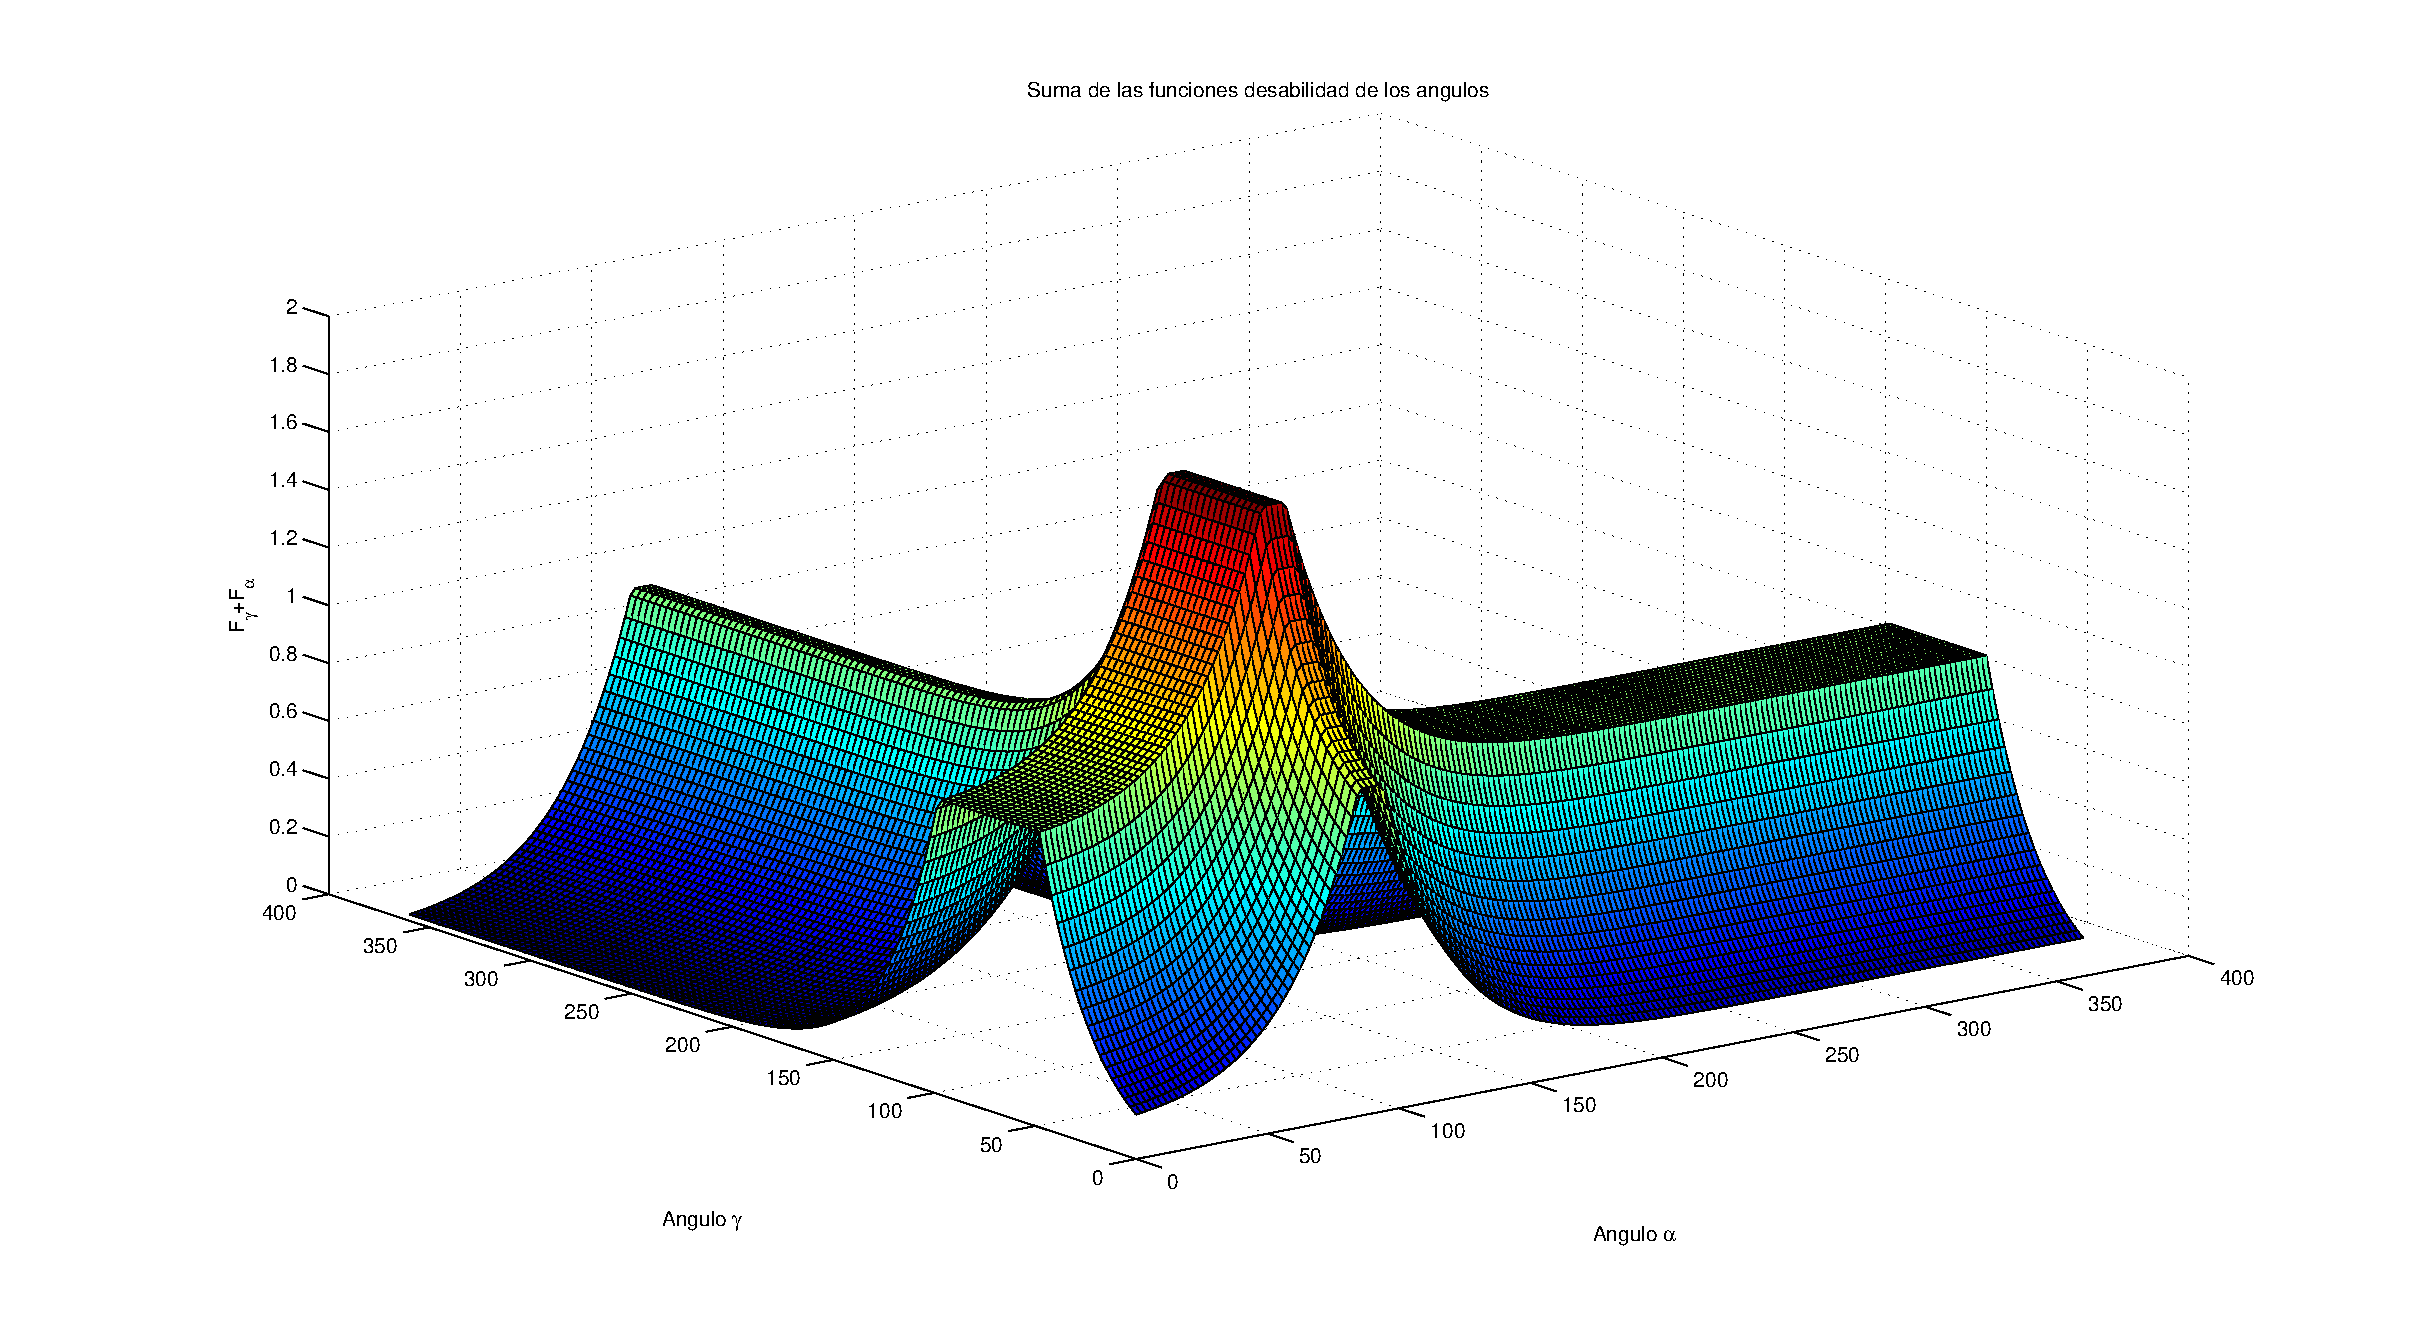
\includegraphics[height=9cm,angle=0]{fdeseabilidadsuma.eps}
\caption{Suma de las funciones deseabilidad tipo Derringer de los \'angulos 
internos del tri\'angulo unitario}
\end{figure}
%%%%%%%%%%%%%%%%%%%%%%%%%%%%%%%%%%%%%%%%%%%%%%%%%%%%%%
La suma de las funciones deseabilidad para los dos \'angulos ($d_{\alpha}$ y 
$d_{\gamma}$) calculados por el AG se muestra en la figura 3.2.
%~\ref{fig1}.


Para encontrar las matrices de masa de los quarks compatibles con los datos 
experimentales se utliza AG para optimizar la funci\'on  deseabilidad, $F_d$,
que es la suma de las doce funciones individuales
$$F_d=\sum^{12}_{i=1}d_i+d_J+d_{\alpha}+d_{\gamma},$$
y tiene un valor m\'aximo de 12, justo cuando los doce par\'ametros que se
intentan ajustar est\'an dentro del intervalo experimental.  

